\documentclass{article}

% if you need to pass options to natbib, use, e.g.:
% \PassOptionsToPackage{numbers, compress}{natbib}
% before loading nips_2016
%
% to avoid loading the natbib package, add option nonatbib:
% \usepackage[nonatbib]{nips_2016}

%\usepackage{nips_2016}

% to compile a camera-ready version, add the [final] option, e.g.:
 \usepackage[final]{nips_2016}

\usepackage[utf8]{inputenc} % allow utf-8 input
\usepackage[T1]{fontenc}    % use 8-bit T1 fonts
\usepackage{hyperref}       % hyperlinks
\usepackage{url}            % simple URL typesetting
\usepackage{booktabs}       % professional-quality tables
\usepackage{amsfonts}       % blackboard math symbols
\usepackage{nicefrac}       % compact symbols for 1/2, etc.
\usepackage{microtype}      % microtypography
\usepackage{graphicx}

\title{Hubble's Tuning Fork: \\A Machine Learning Approach}

% The \author macro works with any number of authors. There are two
% commands used to separate the names and addresses of multiple
% authors: \And and \AND.
%
% Using \And between authors leaves it to LaTeX to determine where to
% break the lines. Using \AND forces a line break at that point. So,
% if LaTeX puts 3 of 4 authors names on the first line, and the last
% on the second line, try using \AND instead of \And before the third
% author name.

\author{
  Brandon Bergerud \\
  Department of Physics and Astronomy\\
  University of Iowa\\
  Iowa City, IA  52242 \\
  \texttt{brandon-bergerud@uiowa.edu} \\
  %% examples of more authors
  \And
  Ossian Mogensen \\
  Department of Computer Science \\
  University of Iowa \\
  Iowa City, IA  52242 \\
  \texttt{ossian-mogensen@uiowa.edu} \\
  %% \AND
  %% Coauthor \\
  %% Affiliation \\
  %% Address \\
  %% \texttt{email} \\
  %% \And
  %% Coauthor \\
  %% Affiliation \\
  %% Address \\
  %% \texttt{email} \\
  %% \And
  %% Coauthor \\
  %% Affiliation \\
  %% Address \\
  %% \texttt{email} \\
}

\begin{document}
% \nipsfinalcopy is no longer used

\maketitle

\begin{abstract}
With the introduction of powerful telescopes such as the Hubble Space Telescope, vast quantities of high-fidelity imagery of remote galaxies have become available. Manual analysis of these images by experts has become infeasible, spawning citizen science projects such as Galaxy Zoo. However, the next generation of telescopes are expected to generate enormous volumes of data, going far beyond the capacity even of crowdsourced volunteers. In this study, we will extend the work done on automatic galaxy image classification in the Galaxy Zoo Kaggle challenge by developing a mapping between the various Galaxy Zoo "classification trees" and the popular Hubble Tuning Fork model. We will build a convolutional neural network to classify galaxies by leveraging the various crowdsourced Galaxy Zoo "gold standard" datasets. The model will be tested against expert-annotated classifications using third-party images.
\end{abstract}

\section{Introduction}
The size and scope of astronomy datasets has increased dramatically in recent years. The introduction of telescopes such as the Hubble Space Telescope (HST) and projects like the Sloan Digital Sky Survey (SDSS) have given astronomers access to imagery of millions of celestial objects. Traditional methods of data analysis, manually inspecting and classifying celestial objects, have become untenable in the face of this embarrassment of riches of data. 

Astronomers have successfully turned to citizen science projects such as Galaxy Zoo to leverage vast numbers of volunteers to help classify objects. The human visual system can, with little effort or training, provide image recognition capabilities that match or exceed the state of the art in computer image recognition. 

With the dawn of a new generation of telescopes, astronomy is threatened to be deluged in a sea of data. The GAIA spacecraft will produce a 3D map of over 1 billion astronomical objects \citep{2016A&A...595A...1G}. The Thirty Meter Telescope (TMT) \citep{2015RAA....15.1945S} and the 40-meter European Extremely Large Telecope (E-ELT) will view the visible universe at unprecedented depth. The Large Synoptic Survey Telescope (LSST) is estimated to generate 15 TB of data each night as it surveys the entire sky \citep{2009AAS...21346003I}. Even these vast sums of data pale in comparision to the output expected from the monsuvian Square Kilometer Array (SKA). Such enormous sums of data are beyond the ability of crowdsourcing to handle: they can only be handled by leveraging supercomputers, sophisticated algorithms, and machine learning.

The Galaxy Zoo Kaggle challenge was a competition in 2013 to produce a machine learning model that could replicate the classifications of citizen science volunteers on a dataset of 70,000 galaxy images captured by HST. The top models performed very well in this challenge, but several questions remain. Can the galaxy classification scheme used by Galaxy Zoo 2 (GZ2) (Figure \ref{fig:GZ2tree}) be effectively mapped to astronomical classification schemes such as Hubble's Tuning Fork, or the more complex de Vaucouleurs system? Will machine learning models trained on the Galaxy Zoo dataset generalize well to other sources? 


\begin{figure}[h]
  \centering
	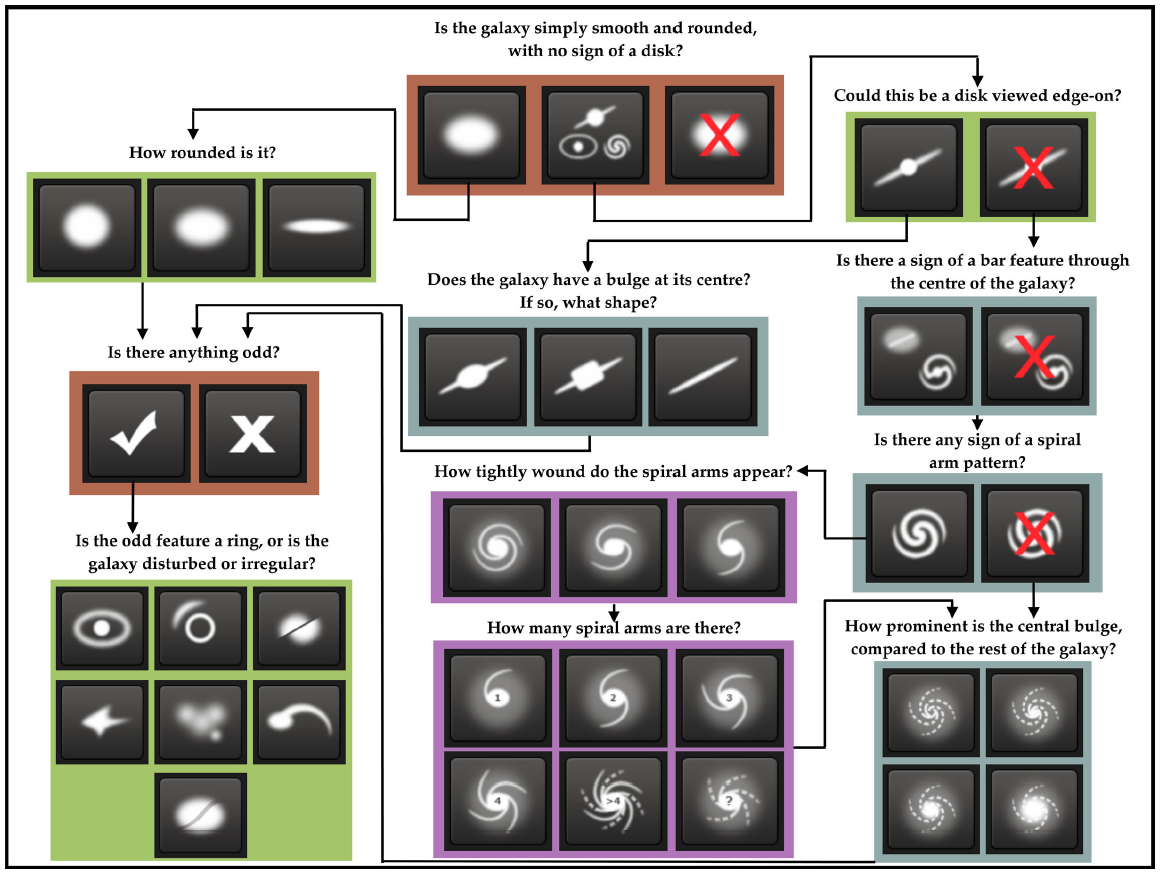
\includegraphics[width=100mm]{../img/GZ2_tree.png}
  \caption{The Galaxy Zoo 2 decision tree. Image from \cite{2013MNRAS.435.2835W}.}
  \label{fig:GZ2tree}
\end{figure}

To answer these questions, we will develop a mapping system between the various Galaxy Zoo “decision tree” classification schemes and the Hubble Tuning Fork scheme (Figure \ref{fig:tuningFork}). We will develop a machine learning system to produce Tuning Fork classifications and train it on data from the Galaxy Zoo projects. We will then locate 3rd party datasets of expert-annotated galaxy images and test our system on these images. This project will investigate the generalizability of the Galaxy Zoo training data and the feasibility of mapping between the two galaxy classification schemes. 

\begin{figure}[h]
  \centering
	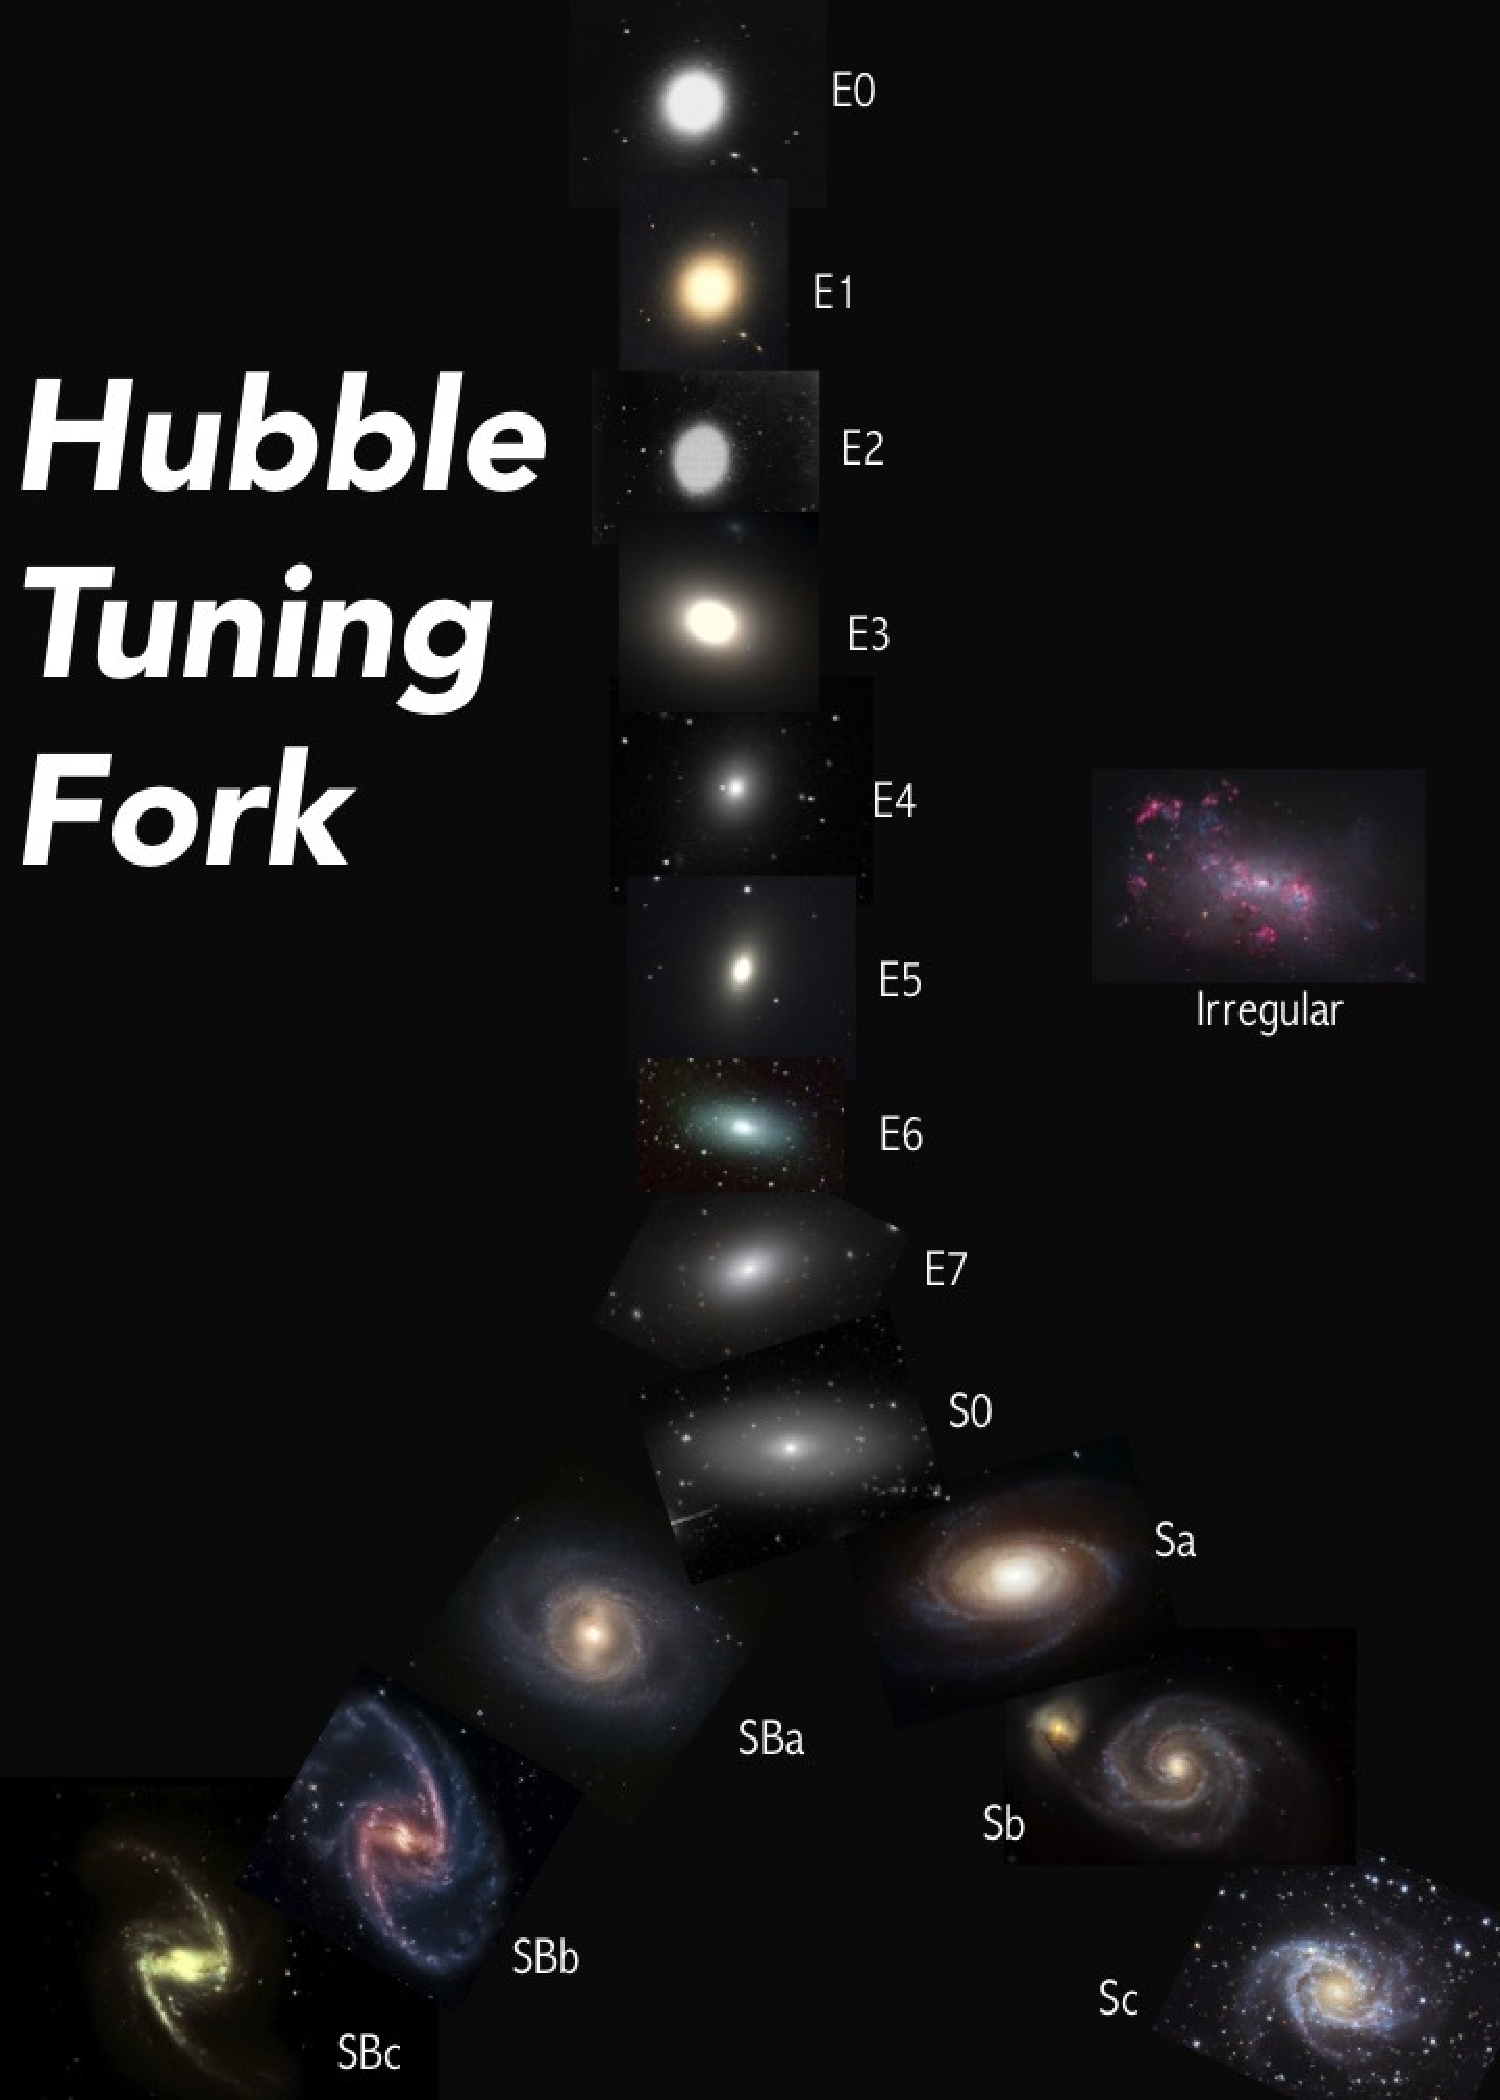
\includegraphics[width=100mm]{../img/tuningFork.pdf}
  \caption{Hubble's tuning fork model. From http://ay17-chusic.blogspot.com/2015/10/20-hubble-tuning-fork.html}
  \label{fig:tuningFork}
\end{figure}


\section{Related Work}
\label{gen_inst}
In the astronomical community, the few automated galaxy classification systems have relied on more tradition methods, focusing on aggressive feature extraction algorithms making use of domain knowledge (such as WND-CHARM) to identify relationships among galaxies. These, however, have tended to focus on the more narrow classification of spirals and ellipticals, occasionally including edge-on spirals and irregular galaxies, and often work with much smaller datasets (see \citealt{2015MNRAS.450.1441D} for a discussion). \cite{2016ApJS..223...20K} were rather unique when they made use of the ``super clean" galaxies from the Galaxy Zoo 1 catalog \citep{2008MNRAS.389.1179L} to classify 3 000 000 galaxies into spirals and ellipticals.

While the top methods achieve $\sim95\%$ accuracy when separating ellipticals and spirals, they tend to perform much worse when the number of categories increases \citep{2004MNRAS.349...87D}.

%One example of the simple classification approach was done by \cite{2016ApJS..223...20K}, who, rather uniquely, made use of the ``super clean" galaxies from the Galaxy Zoo 1 catalog \citep{2008MNRAS.389.1179L} to classify 3 000 000 galaxies into spirals and ellipticals.

\cite{stanford}, students in Prof. Ng's machine learning class at Stanford, recently looked at several machine learning methods for classifying galaxies using the GZ2 dataset. While acknowledging the difficulty of directly classifying to the Hubble types, they sought to bridge the gap by modeling certain features, such as "roundness" and "diskiness". They utilized the GZ2 decision tree to assign each galaxy to one of five categories: disc, spiral, elliptical, round, and other. In their preprocessing stage, images were cropped to reduce the file size, as well as reduce the number of nearby sources contaiminating the images. The galaxies were then rotated to align the principle axis, before proceeding with a background subtraction.

To further reduce the dimensionality of the problem, the authors applied principal component analysis (PCA), selecting the top 125 components to maintain $>99\%$ of the variance. To classify the galaxies, they utilized a support vector machine (SVM) with a radial basis function (RBF) kernel, a decision tree, random forest, k-nearest neighbors, and an AdaBoost classifier, determing the classification accuracy using 10-fold cross validation. Overall, random forest produce the best results, achieving 67\% accuracy. The poor success rate lead them to look into predicting probabilities (regression) rather than directly modeling the classes, similar to the Galaxy Zoo Kaggle challenge. They achieved better results in this regard, attaining $\sim 95\%$ accuracy.

Overall, the biggest source of error was misclassifying spiral galaxies into the "other" category, which they attributed to the faintness (low signal-to-noise) of the spiral arms in many images. In addition, examining Figure 3 in their paper and comparing the original image with the 125 PC image, it appears that their method may hinder extracting the spiral arms by smoothing the disk, making classification more difficult. While this may be necessary for more traditional machine learning methods, deep learning can deal directly with the large feature space.


The Galaxy Zoo Kaggle challenge showed the power of convolutional neural networks (CNNs) when it comes to galaxy classification. Rather than relying on domain knowledge, the models had to learn to identify features on their own and were able to successfully reproduce the probabililty distributions of the citizen scientists. The processing pipeline for the top performing model \citep{2015MNRAS.450.1441D} is schematically illustrated in Figure \ref{fig:GZ2_network}, which we shall examine next. 

The winning algorithm was an ensemble method, averaging the results of many different CNNs. In the pre-processing stage, the image was cropped and rescaled several times down to $69 \times 69$ pixel images, which occasionally removed part of the galaxy. In some of their models, they used SExtractor to estimate the position and size of the galaxy, allowing them to center and rescale the galaxies to a standardized size. In addition, gray-scaling was examined, although this lead to worse results.

Due to the limited sample size, the number of images was increased by performing random pertubations, such as rotating, translating, scaling, and flipping, as well adjusting the color brightness on demand so that the model was never trained on the exact image twice. In addition, the number of images was increased by rotating, flipping and cropping each image into 16 different, but overlapping, $45 \times 45$ pixel images respresenting different viewpoints. Each of the 16 images were then passed together through the CNN, which performed several convolutions and pooling before concatenating the results and passing through a couple fully connected layers to output the final categorical probabilities. The probabilities were then averaged over 17 models.

Overall, the model did quite well, achieving $\sim 99\%$ accuracy. It stuggled most with the larger angular sized galaxies (more nearby), as well as those that were not radially symmetric.


\begin{figure}[h]
  \centering
	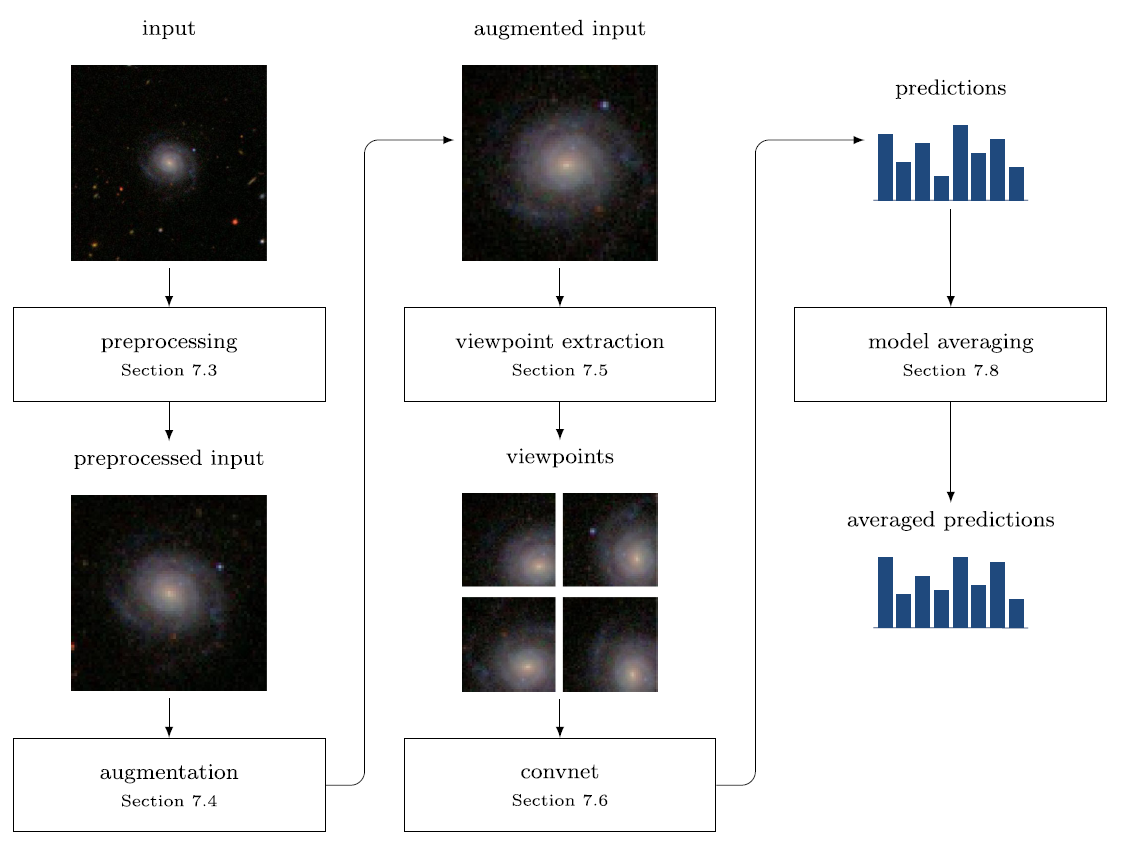
\includegraphics[width=130mm]{../img/GZ2_network.png}
  \caption{Processing pipeline for the top model in the Galaxy Zoo Kaggle competition. From \cite{2015MNRAS.450.1441D}.}
  \label{fig:GZ2_network}
\end{figure}




\section{The Proposed Work}
As dicussed earlier, the existing systems from the Galaxy Zoo Kaggle challenge do an excellent job of replicating the voting patterns of citizen science volunteers on the Galaxy Zoo 2 dataset. However, it would be useful to develop an automated system based on the large annotated Galaxy Zoo datasets to classify new imagery from other sources using the popular Hubble Tuning Fork scheme. While this can be done to some extent using the kaggle models, it requires cross-correlating expertly annoted images to find the optimal probability cutoffs to transform the probability distributions to Hubble T-types, adding an additional layer of complexity that the machine wasn't required to learn. We will develop a mapping between the two classification schemes and develop such a machine learning system to directly classify images. 

Our model will differ slightly from the format of the Kaggle challenge. The Kaggle Galaxy Zoo challenge formulated the problem as a regression on the class probabilities, defined as the ratio of citizen science volunteers that gave a given galaxy a certain classification. To match the structure of our gold standard Tuning Fork scheme data, we will instead treat this as a classification problem and select only those galaxies whose vote fractions are within our chosen threshold for each Hubble type. This will favor the more nearby galaxies, whose properties the top performing model in the Kaggle competition had a harder time predicting accurately, hopefully, leading to an improvement in that regard. In addition, it would serve as a more interactive tool that could serve as a complement to the galaxy classification lab in \emph{Stars, Galaxies, and the Universe}.

Based on prior work, the best approach to galaxy classification appears to be a Deep Convolutional Neural Network. The top image recognition CNNs in recent years have used the inception model \citep{2014arXiv1409.4842S} as a building block in their networks (Figure \ref{fig:inception}). We will follow this trend.

\begin{figure}[h]
  \centering
	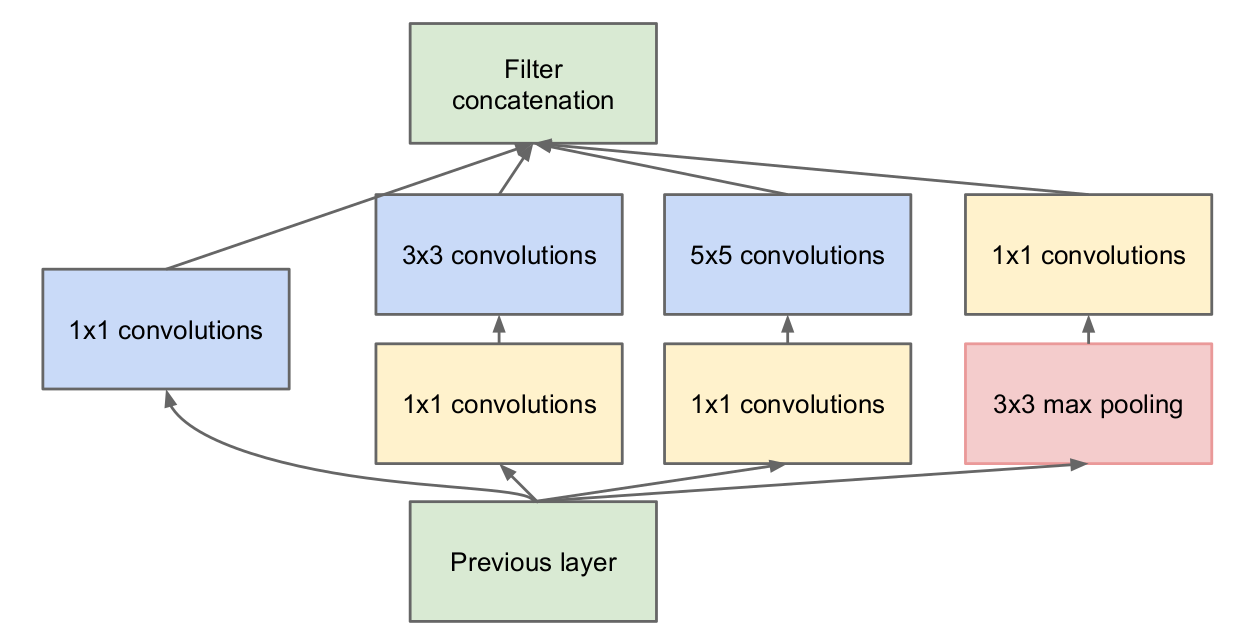
\includegraphics[width=100mm]{../img/inception.png}
  \caption{Inception block. The top image recognition CNNs in recent years use many inception blocks in their networks. From \cite{2014arXiv1409.4842S}.}
  \label{fig:inception}
\end{figure}

Since many of the images used in Galaxy Zoo 2 had poor consensus among the citizen scientists, we will attempt to achieve better results by incorporating the results from Galazy Zoo 1, Galazy Zoo: Hubble, and Galaxy Zoo: CANDELS, and pruning the dataset. Galaxy Zoo 1, which is the largest of the datasets, will be mostly inadequate for classification purposes as it aimed at determining whether a galaxy was a spiral, elliptical, edge-on disk, or a merging system (irregular). It will, however, provide a good dataset for initial testing to verify that we can separate the basic mophologies. The three remaining Galaxy Zoo projects asked similar questions, allowing for similar mapping schemes to the Hubble tuning fork.



\section{Plan}
Our project can be broken into several stages:
\begin{enumerate}
\item	Map the Galaxy Zoo classication results to the Hubble types and prune the results
\item	Build the CNN and test on images from the GZ1 dataset
\item	Begin training on the tuning fork dataset and fine-tune the model architecture
\item	Test the model on third-party images
\end{enumerate}

The mapping of the galaxy zoo classification results can be done fairly quickly, the only issue maybe the downloading time from the SDSS database. In addition, the size of the sample may prove to be an issue. With limited time we may be force to work with a smaller subset than would be desired. 

For building the CNN, we will use the python module Keras with the Tensorflow backend. Since CNNs are computationally expensive, we will attempt to gain access to the GPUs on one (or both) of the Iowa clusters to reduce the computation time. Tensorflow is designed to make use of GPUs if present, thus requiring no additional programming on our part.

After our final model has been trained, we will test its generalizability by using third party images of nearby galaxies and testing the classification results. Images taken with the Iowa Robotic Observatory could be one such third party source. In Figure \ref{fig:M51}, an unfiltered image of the Whirlpool Galaxy taken by the University of Iowa's Gemini telescope is shown. The Whirlpool Galaxy is a type Sb on Hubble's Tuning Fork. 

A general time table for our project is given in the table below:

\begin{table}[!h]
  \caption{Project Schedule}
  \label{tab:plan}
  \centering
  \begin{tabular}{ll}
    \toprule
    %\multicolumn{2}{c}{Part}                   \\
    \cmidrule{1-2}
    Week     & Tasks \\
    \midrule
    03 April 	& GZ1 download; building CNN    \\
    10 April    & Download full dataset; testing CNN on simpler scheme \\
    17 April    & Tuning CNN on full tuning fork; begin writing report       \\
	24 April	& Finish CNN work; prepare presentation; continue writing report  \\
	01 May		& Presentation; finish report \\
    \bottomrule
  \end{tabular}
\end{table}


Preprocessing could be a valuable tool for improving the results, although the limited time requirements may prevent us from exploring this option in depth. We'll likely crop the images to reduce computation time, and if needbe we could apply some affine transformations to increase the size of our dataset. An intricate method, similar to the one utilized by \cite{2015MNRAS.450.1441D}, could be a future implementation.


When it comes to the overall accuracy, we hope to achieve performances at least comparable to previous studies when it comes to getting the most basic morphological shapes such as spirals vs ellipiticals $(\sim 95\%)$. With regard to subclassifications, which are somewhat subjective, we anticipate getting large errors, but hope to achieve accuracies that are significantly greater than random guessing. Ideally, our model should also give fairly similar Hubble types among the most likely categories (e.g., having E5 and E6 as the two top predictions, rather than E0 and E7).


\begin{figure}[h]
  \centering
	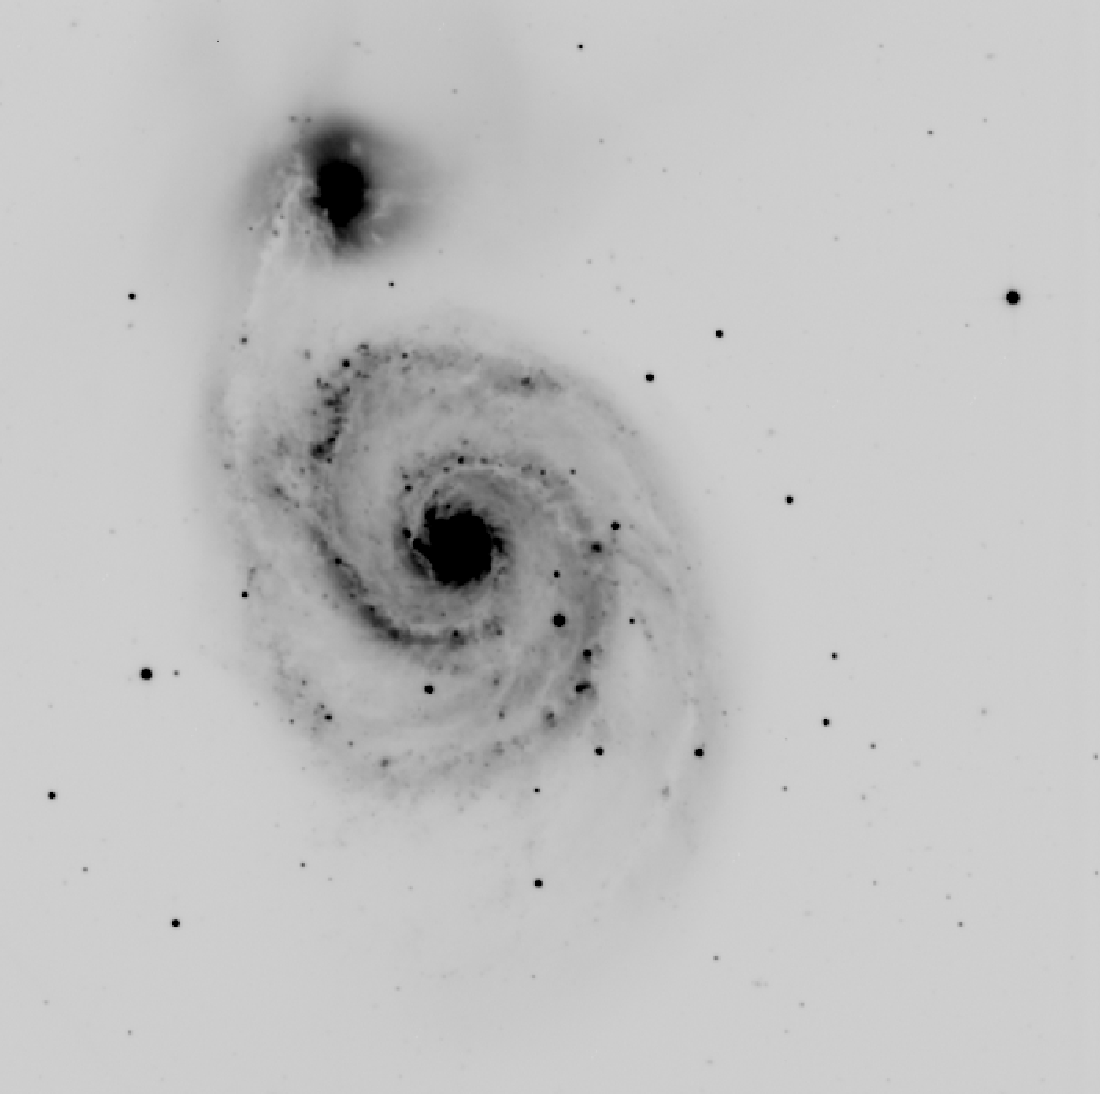
\includegraphics[width=100mm]{../img/M51.pdf}
  \caption{Unfiltered image of the Whirlpool Galaxy (Sb). Taken with the Iowa Robotic Observatory.}
  \label{fig:M51}
\end{figure}

\subsubsection*{Acknowledgments}

We would like to acknowledge the work of the Galaxy Zoo team and the countless citizen volunteers in collecting and annotating the massive Galaxy Zoo dataset that makes this work possible. 


\begin{thebibliography}{9}
\bibitem[de la Calleja \& Fuentes(2004)]{2004MNRAS.349...87D} de la Calleja, J., \& Fuentes, O.\ 2004, MNRAS, 349, 87 
\bibitem[Dieleman et al.(2015)]{2015MNRAS.450.1441D} Dieleman, S., Willett, K.~W., \& Dambre, J.\ 2015, MNRAS, 450, 1441
\bibitem[Gaia Collaboration et al.(2016)]{2016A&A...595A...1G} Gaia Collaboration, Prusti, T., de Bruijne, J.~H.~J., et al.\ 2016, Astronomy and Astrophysics, 595, A1  
\bibitem[Gauthier et al.(2016)]{stanford} Gauthier, A., Jain, A., Noordeh, E.\ 2016
\bibitem[Ivezic et al.(2009)]{2009AAS...21346003I} Ivezic, Z., Tyson, J.~A., Axelrod, T., et al.\ 2009, Bulletin of the American Astronomical Society, 41, 460.03 
\bibitem[Kuminski \& Shamir(2016)]{2016ApJS..223...20K} Kuminski, E., \& Shamir, L.\ 2016, ApJS, 223, 20 
\bibitem[Lintott et al.(2008)]{2008MNRAS.389.1179L} Lintott, C.~J., Schawinski, K., Slosar, A., et al.\ 2008, MNRAS, 389, 1179
\bibitem[Skidmore et al.(2015)]{2015RAA....15.1945S} Skidmore, W., TMT International Science Development Teams, \& Science Advisory Committee, T.\ 2015, Research in Astronomy and Astrophysics, 15, 1945 
\bibitem[Szegedy et al.(2014)]{2014arXiv1409.4842S} Szegedy, C., Liu, W., Jia, Y., et al.\ 2014, arXiv:1409.4842 
\bibitem[Willett et al.(2013)]{2013MNRAS.435.2835W} Willett, K.~W., Lintott, C.~J., Bamford, S.~P., et al.\ 2013, MNRAS, 435, 2835  
\end{thebibliography}


\end{document}
